\section{Subtraktion $n$-stelliger ganzer Zahlen}

Wir wollen möglichst die gleiche Hardware für die Subtraktion wie für die Addition verwenden. Dabei können wir uns zu Nutze machen, dass gilt:
\begin{align}
	a-b=a+\underbrace{(-b)}_{\text{2er Komplement}}=a+\underbrace{(\overline{b})}_{\text{1er Komplement}}+1\notag
\end{align}
Damit wird auch in der hinteren Postion ein Volladdierer benötigt und Addition und Subtraktion laufen über die gleiche Hardware.

Zugleich optimieren wir noch die Addierer. Vom Carry-Ripple-Adder zum \begriff{Carry-Lookahead-Adder} und dann zum \begriff{Carry-Skip-Adder}. Während der Carry-Ripple-Adder eine Komplexität von $T(n)=\mathcal{O}(n)$ hat, hat der Carry-Lookahead-Adder eine Komplexität von $T(n)=\mathcal{O}(\log_2 n)$

\begin{figure}[ht]
	\centering
	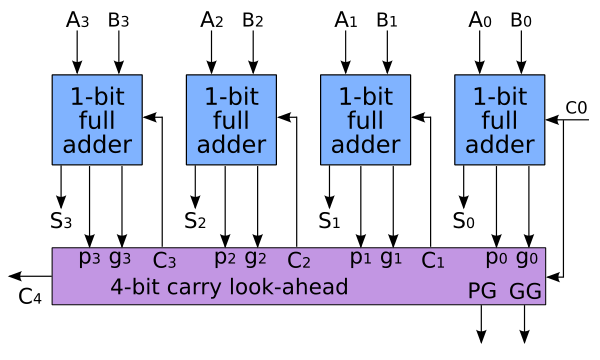
\includegraphics[width=10cm]{images/Carry-Lookahead-Adder_2.png}
	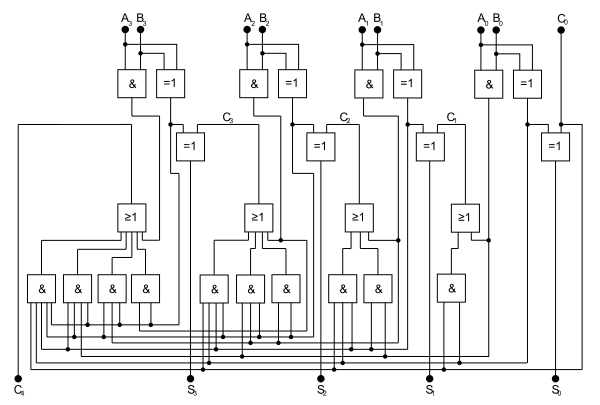
\includegraphics[width=10cm]{images/Carry-Lookahead-Adder.png}
	\caption{Carry-Lookahead-Adder}
\end{figure}

\begin{figure}[ht]
	\centering
	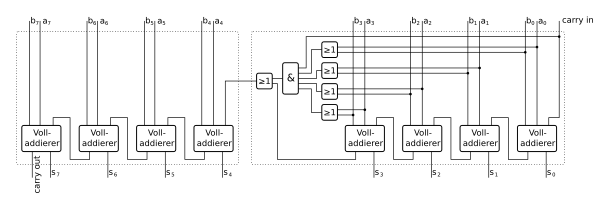
\includegraphics[width=10cm]{images/Carry-Skip-Adder.png}
	\caption{Carry-Skip-Adder}
\end{figure}